\documentclass[11pt]{article}
\usepackage[margin=1in]{geometry}
\usepackage{amsmath,amssymb}
\usepackage{graphicx}
\usepackage{float}
\usepackage{subcaption}

\title{Meeting}
\begin{document}
\maketitle
\section{Updates}
  \begin{itemize}
    \item I finished implementing their method. The contracts designed by the model I trained look similar to the ones in the paper. There are still some discrepancies with regards to the data that I haven't been able to figure out, but I think right now would be a good time to email the authors with our questions. 
    \item The next step will be to start training simpler models to compare our method to theirs. 
  \end{itemize}

  \begin{figure}[H]
    \centering
      \begin{subfigure}[b]{0.47\textwidth}
        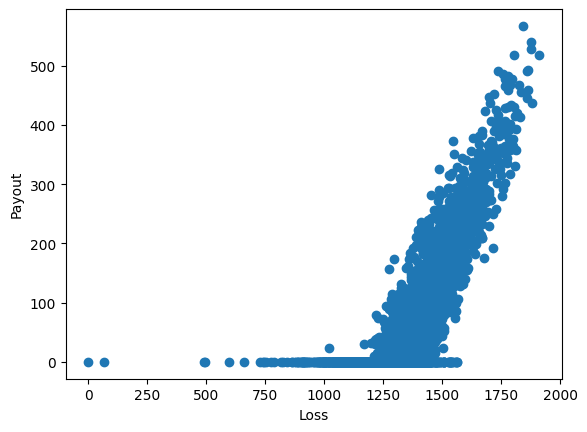
\includegraphics[width=\textwidth]{..//../../output/figures/Chen_Replication/NN_payout.png}
    \caption{Contract from my replication}
        \label{fig:f1}
      \end{subfigure}
     \hfill
      \begin{subfigure}[b]{0.47\textwidth}
        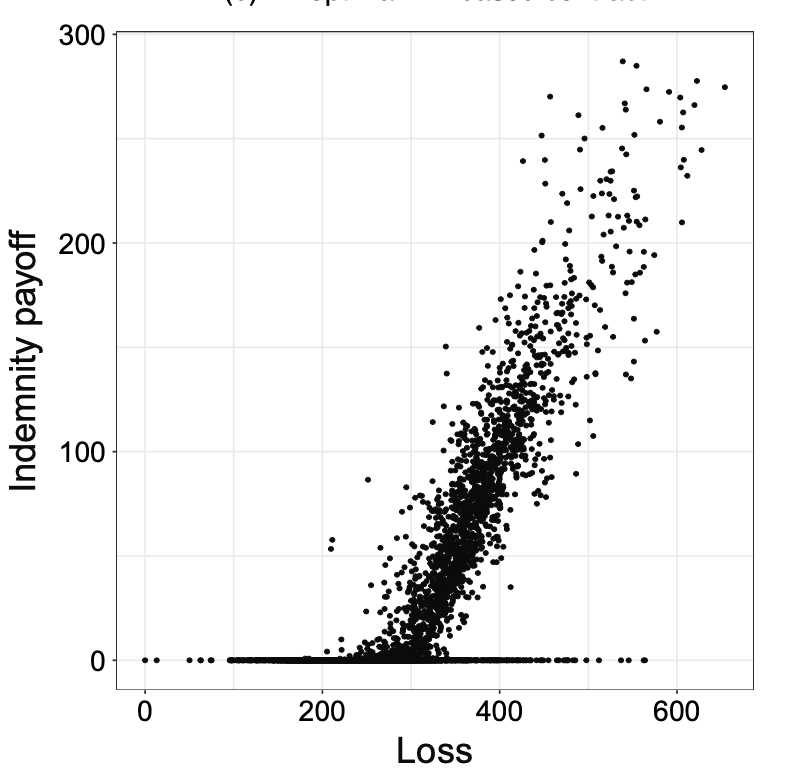
\includegraphics[width=\textwidth]{..//../../output/figures/Chen_Replication/Chen_payout.png}
    \caption{Contract from Chen et al 2023}
        \label{fig:f2}
      \end{subfigure}
      \caption{Replication Plots}
    \end{figure}






  \subsection{Replication Notes}
    \begin{enumerate}
        \item The first discrepancy in replicating comes from detrending the yield data. In the paper they say they detrended the data using a second order polynomial fit with a robust regression method. I have tried every robust regression method available in the most popular Python ML library, but the detrended values do not match up. The average loss in their detrended data is 284.6, however amongst the methods I tried, the one with the smallest mean had a mean of 843.
        \item Another data discrepancy is that they have 7869 observations. It's not included in the code, but from the data, it appears that they fit a separate trend polynomial for each county, and used these fitted trends to adjust all values to 2018 values. However, the data they said they used is missing data 2018 data for 7 counties. That means that you have to throw away the data from these counties, because you can't express it in 2018 values. These reduces the total number of observations to 7227. 
        \item In their code, they train the neural network for 100 epochs, however, when I trained it for 100 epochs the contracts looked pretty different. The contracts didn't start looking similar until I trained the model for 300+ epochs. I suspect this has to do with the discrepancy in the detrended data, their detrended values have much lower variance (6500 vs 20,000).
        \item The implementation of their algorithm differs from what they describe in the appendix, but I'm not sure if this is worth flagging. What differs is the conditions in the while loop. In the paper, they have $|I-I_{\text{last}}| > \epsilon_1 \text{or} g(I) > \epsilon_2 \text{or} |\pi(I)-\pi(I_{\text{last}})| > \epsilon_3$, whereas in the code they have $(g(I) > \epsilon_1 \text{or} \frac{|\pi(I)-\pi(I_{\text{last}})|}{\pi(I_{\text{last}})}) \text{and} \phi < \epsilon_4$.
    \end{enumerate}
  

\end{document}